\documentclass[10pt,a4paper,]{article}
\usepackage{ucs}
\usepackage[T1]{fontenc}
\usepackage[utf8x]{inputenc}
\usepackage[serbian]{babel}
\usepackage{amsmath}
\usepackage{amsfonts}
\usepackage{amssymb}
\usepackage{graphicx}
\usepackage{xcolor}
%\usepackage[OT2]{fontenc}
\title{Skripta iz Uvoda u teoriju uzoraka}

\begin{document}
\maketitle

\section{nedelja}
\subsection{Naučno istraživanje}
\textbf{Naučno istraživanje} je sistematsko, plansko i objektivno ispitivanje nekog problema, prema određenim metodološkim pravilima, čija je svrha da se pruži pouzdan i precizan odgovor na unapred postavljeno pitanje.
\\[0.1cm]

Može se shvatiti kao kritički, kontrolisani i ponovljivi proces sticanja novih znanja, neophodnih (a ponekad i dovoljnih) za identifikovanje, određivanje i rešavanje naučnih (teorijskih i empirijskih) problema.
\\[0.1cm]

\textbf{Teorijsko} istraživanje vs Empirijsko (\textbf{iskustveno})
istraživanje.
\\[0.3cm]

Svako naučno istraživanje ima više međusobno logično povezanih faza. 
\\
\textbf{Faze} su:
\begin{itemize}
	\item identifikovanje i određivanje problema

	\item određivanje cilja istraživanja
	\item definisanje ključnih izraza
	\item postavljanje hipoteze i izvođenje logičkih posledica iz hipoteze
	\item izbor istraživačke strategije i plana istraživanja
	\item razvijanje mernih i drugih instrumenata istraživanja
	\item određivanje onovnog skupa (populacije) i odabir uzorka
	\item sprovođenje istraživanja i prikupljanje relevantnih podataka
	\item obrađivanje i analiza podataka dobijenih istraživanjem
	\item tumačenje rezultata istraživanja i izvođenje zaključ(a)ka
	\item izrada izveštaja o obavljenom istraživanju
	\item prezentacija rezultata istraživanja


\end{itemize}
\subsection{Osnovni pojmovi}
\textbf{Entitet}/\textbf{jedinica posmatranja} (en. 'observation
unit') - živo biće ili objekat čija su svojstva predmet istraživanja.

\textbf{Populacija} ('population') - skup / kolekcija entiteta.
\\[0.1cm]
Na osnovu broja entiteta, tj. \textbf{obima} 
/ veličine \textbf{populacije} ('populationsize') 𝑁, može biti:
\begin{itemize}
           \item konačna populacija−𝑁 je prirodan broj
           \item beskonačna populacija−𝑁→+∞
\end{itemize}
Trebalo bi razlikovati:
\begin{itemize}
        \item ciljnu populaciju('target population')
        \item populaciju na kojoj se efektivno sprovodi 
           istraživanje ('study population')
           \footnote{Nadalje se pretpostavlja: 
           target population = study population i 𝑁<+∞}
\end{itemize}


\textbf{Uzorak} ('sample') - podskup populacije; sadrži izvesne entitete koji potiču iz populacije, na bazi čijeg proučavanja će se izvoditi zaključci o čitavoj populaciji
\\
\textbf{Obim uzorka} ('samplesize') n 
\footnote{\underline{Uvek} konačna vrednost} 
\\
\textbf{Jedinica uzorkovanja} ('sampling unit')
\footnote{U opštem slučaju nije isto što i jedinica posmatranja, koja 
predstavlja osnovni objekat posmatranja i prikupljanja informacija. 
Jedinice uzorkovanja su međusobno disjunktni skupovi entiteta}
\\
\textbf{Okvir za odabir uzorka} ('sampling frame') - popis (ili neka druga specifikacija) svih jedinica uzorkovanja
\\[0.25cm]
Npr. svakoj jedinici uzorkovanja pridruži se različit prirodan broj (počevši od 1). Ti brojevi nazivaju se \textbf{oznake jedinica},
služe za njihovo identifikovanje i ostaju nepromenjeni 
sve do kraja istraživanja.
\\

\underline{Primer} - telefonsko istraživanje biračkog tela.
\\[0.1cm]
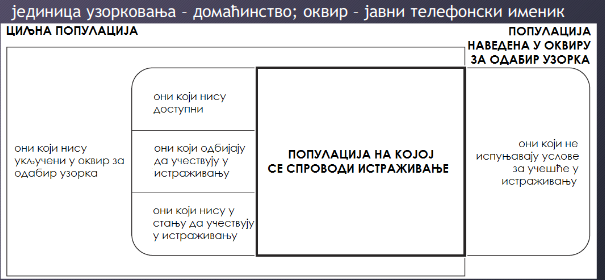
\includegraphics[scale=0.5]{primer1}
\\[0.2cm]
Zašto uzorkovanje?
\\
\textbf{Potpuno} ispitivanje populacije 
(proučavanje tzv. \textbf{cenzusa}) je, u 
mnogim  slučajevima, neracionalno ili čak principijelno nemoguće. 
Čak i onda kada postoji mogućnost potpunog ispitivanja populacije 
istraživač se obično opredeljuje za \textbf{delimično} ispitivanje (proučavanje 
uzorka) jer je (u odnosu na potpuno ispitivanje):

\begin{itemize}
	\item jeftinije 
	\item brže
	\item kontrola tačnosti prikuplenih podataka je jednostavnija
	 i lakša
\end{itemize}

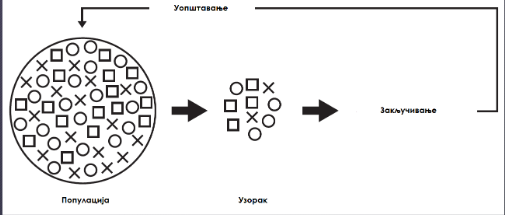
\includegraphics[scale=0.55]{primer2}
\\[0.25cm]

Termin populacija odnosi se na skup entiteta istovrsnih u odnosu 
na jedno ili više zajedničkih svojstava, koja se mogu posmatrati. 
Ipak, entiteti, iako \textbf{istovrsni}, \textbf{nisu istovetni}.
\\ 
Određivanje populacije 
predstavlja značajnu i, neretko, tešku fazu istraživanja. Populacija 
mora biti definisana: pojmovno (u smislu svog sadržaja - šta su 
entiteti, a šta jedinice uzorkovanja?), prostorno i vremenski.

\textbf{Obeležje} ('study variable') - posmatrana zajednička 
karakteristika 
svih entiteta u populaciji, tj. preciznije, izvesno varijabilno 
svojstvo od interesa, koje je određeno za svaki entitet u populaciji.
\footnote{Obeležje najčešće nije neko od definicionih svojstava
populacije.}

\subsection{Tipovi obeležja}

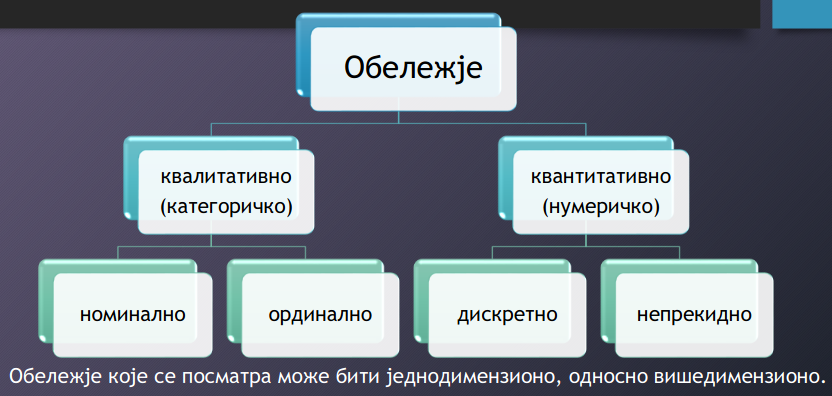
\includegraphics[scale=0.4]{primer3}
\pagebreak
\\
\underline{Primer}: tipovi obeležja
\begin{itemize}
	\item kvalitativna
	\begin{itemize}
		\item nominalna
			\begin{itemize}
				\item boja očiju, krvna grupa
				\item etnička / verska pripadnost 
				\item radna mesta na fakultetu
				\item raspoloženje građana Srbije prema pristupanju
				u EU
				\item posedovanje profila na društvenim mrežama
			\end{itemize}
		\item ordinalna
			\begin{itemize}
				\item nivo akademskih studija
				\item čin oficira u vojsci
				\item ocena restorana na Tripadvisor
				\item stanje pacijenta
				\item intezitet bola
			\end{itemize}
	\end{itemize}
	\item kvantitativna
	\begin{itemize}
		\item diskretna
			\begin{itemize}
				\item broj stanovnik sa pravom glasa u određenoj
				opštini
				\item broj blizanaca rođenih u toku godine u
				određenoj regiji
				\item broj kućnih ljubimaca u domaćinstvu
			\end{itemize}
		\item neprekidna
			\begin{itemize}
				\item visina, težina, starost, IQ
				\item dužina lista određene biljne vrste
				\item koncetracija soli u morskoj vodi
			\end{itemize}
	\end{itemize}
\end{itemize}

\underline{Primer}: populacija i obeležje
\begin{itemize}
\item 
\textcolor{red}{Populacija}: skup studenata koji su upisali Uvod u teoriju uzoraka školske 2019/20. godine.
\\
\textcolor{blue}{Obeležje}: pol; broj položenih ispita, broj položenih ESPB bodova,prosečna ocena svih položenih ispita –zaključno sa rokom Januar 2 ove školske godine; ocena na kursu Statistika
\item
\textcolor{red}{Populacija}: skup svih poljoprivrednih gazdinstava u Srbiji(referentni period–oktobar/novembar2018)
\\
\textcolor{blue}{Obeležje}:površina korišćenog poljoprivrednog zemljišta;
broj grla stoke; primenjeni proizvodni metodi

\item
\textcolor{red}{Populacija}: skup svih domaćinstava u regionu Šumadije i Istočne Srbije(referentni period –2017. g)
\\
\textcolor{blue}{Obeležje}: lična potrošnja domaćinstva (mesečni prosek)

\item
\textcolor{red}{Populacija}: jedna serija LED sijalica izvesnog proivođača.
\\
\textcolor{blue}{Obeležje}: dužina radnog veka sijalice u satima.


\item
\textcolor{red}{Populacija}: skup svih meseci u periodu od 2000. do 2016. g.
\\
\textcolor{blue}{Obeležje}: mesečni broj vetrovitih dana u Vršcu	
\end{itemize}


Obeležje se može shvatiti kao funkcija koja entitetima u populaciji 
pridružuje realne brojeve ili neke druge vrednosti.
\\
Neka je data 
populacija sa 𝑁 jedinica, koje su u okviru za odabiruzorka označene 
brojevima iz skupa $\omega={1,2,...,𝑁}$ (i time jednoznačno određene)i neka 
je 𝑌 obeležje od interesa.Neka je sa $y_k$ označena vrednost obeležja 
𝑌 entiteta označenog sa 𝑘. \\

Zadatak pri istraživanju obično se svodi na donošenje zaključaka o 
(nepoznatoj) vrednosti realne funkcije 
$$\theta=f(y_{1},y_{2},,y_{n})$$, koja se naziva 
\textbf{populacijska vrednost} ('population value') ili 
\textbf{parametar populacije}.
\\

Najčešće funkcije koje se pojavljuju kao parametri populacije:
\begin{itemize}
	\item Kvantitativna obeležja
		\begin{itemize}
			\item populacijska srednja vrednost ('population mean')
			$$m_Y  = m = \frac{1}{N}\sum_{k=1}^{N}y_{K}$$
			\item populacijski total ('population total')
			$$\tau_{Y} = \tau = \sum_{k=1}^{N}y_{K} = Nm_Y $$
			\item populacijska disperzija ('population variance')
			/ standardno odstupanje
			$$\sigma^2_Y = \sigma^2 = 
			\frac{1}{N-1}\sum_{k=1}^{N}(y_K - m_Y)^2$$ i
			$$\sigma_Y = \sigma = \sqrt{\sigma^2_Y}$$
		\end{itemize}
	\item Kvalitativna obeležja
		\begin{itemize}
			\item populacijska proporcija ('population proportion')
			\item populacijska medijana, kvantili, moda...
		\end{itemize}
\end{itemize}

Ideja je da se zaključci o populacijskim vrednostima donose na osnovu 
informacija dobijenih ispitivanjem uzorka.

„Dobar“ uzorak ima osobinu \textbf{reprezentativnosti}. To je uzorak 
koji predstavlja „umanjenu“, a nikako „iskrivljenu“, niti „uveličanu“ 
sliku jednog dela populacije. Uzorak sa ovom osobinom verno odslikava 
strukturu populacije koju predstavlja, „izgledajući“ kao i populacija 
u svim aspektima relevatnim za istraživanje.
\\
\pagebreak
\\
Na reprezentativnost uzorka utiču:
\begin{itemize}
	\item tip uzorka (prema metodu odabira)
	\item veličina uzorka
	\item varijabilnost posmatranog obeležja
\end{itemize}

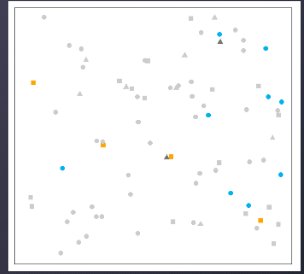
\includegraphics[scale=0.5]{primer4}
\end{document}